\documentclass[11pt]{article}
\usepackage[margin=1in]{geometry}
\usepackage[T1]{fontenc}
\usepackage{lmodern}
\usepackage{microtype}
\usepackage{amsmath}
\usepackage{booktabs}
\usepackage{graphicx}
\usepackage{caption}
\usepackage[section]{placeins}
\usepackage{xcolor}
\usepackage{hyperref}
\hypersetup{colorlinks=true, linkcolor=blue!50!black, urlcolor=blue!50!black}
\usepackage{enumitem}
\setlist{nosep}
\captionsetup{font=small, labelfont=bf}
\graphicspath{{../../results/report-figures/}}
\newcommand{\ttt}[1]{\texttt{\small #1}}

\title{Filler tokens in open models:\\ a screen, a training attempt, and what a dot position is doing}
\author{Nick Rui \\ \small with the DeepSeek V4 Flash results and pipeline by Nicole (the \ttt{extract\_dsv4.py} line of work)}
\date{September 3, 2026}

\begin{document}
\sloppy
\maketitle

\section*{Summary}

Nicole found that DeepSeek V4 Flash solves a two-step variable-binding puzzle 70\% of the time, and 98\% of the time if fifty dots are inserted between the question and the answer. Dots placed before the question do nothing. Her lens and patching work showed the model staging intermediate values in the dot positions, copying them across dots, and reading them back late. The obvious question was whether smaller, open models do the same. They do not, and this report documents how thoroughly they do not.

I ran the same items through ten open models from 4B to 35B parameters (Qwen3, Qwen3.5, Qwen3.6, Llama-3.1, Gemma-3, OLMo-3.1; dense and mixture-of-experts). Every one scores between 0 and 14\% on the two-step items at every dot count, with no placement-specific gain. On an easier one-step variant where they score 50 to 100\%, dots still change nothing. Sampling more answers would not help either: the expected pass@20 barely moves with dots.

I then fine-tuned Qwen3.5-9B with LoRA to solve the task with dots present. Five variants (mixed dot counts, a harder chain, a 4B model, dots-only training, no-dots training) all learn the task, and all learn it as a direct computation at the answer position. The model trained \emph{only} on prompts with dots scores 40/50 with no dots at all. On held-out items, its dot positions decode to the dot token, carry no stage value beyond a faint late leak, can be wiped at every block without changing the answer (median shift 0.02 nats), and receive 1 to 4\% of the answer position's attention. Fine-tuning with dots made the dots more uniform and less attended than in the untrained model. The model learned to route around them.

Running the same anatomy on DeepSeek V4 Flash itself (Part V) shows the mirror image: its answer positions put 16 to 43\% of late-block attention on the dots, the dot residuals are problem-specific and split by hyper-connection stream, and the answer is decodable from the dots but not from the question token. My reading is that using filler as a workspace is a learned habit, not something transformers do given capacity. DeepSeek's reasoning-focused post-training is the most plausible source, with its four-stream residual making the habit cheap to implement. The one experiment that would settle half of this, running the released DeepSeek-V4-Flash-Base checkpoint, needs about 300\,GB of GPU memory that this project did not have.

\tableofcontents

\section{Background}

\subsection{The claim being tested}

The filler-token paper (arXiv:2607.03502) reports that a model's accuracy on some multi-step tasks rises when meaningless tokens are inserted between the question and the answer. The tokens carry no information. If they help, the model must be doing computation in those positions during the forward pass, computation it could not fit into the positions it already had.

The task used throughout is chained variable binding. A prompt lists five definitions, some literal and some referring to an earlier variable, and asks a question that requires resolving one reference. An example from the released set:

\begin{quote}\small\ttt{nof = 97}\\
\ttt{hoz = twice the number for nof minus 21}\\
\ttt{Question: What is twice the number for hoz plus 28?}\end{quote}

The answer needs two hidden steps: $97 \to 194 \to 173$, then $173 \to 346 \to 374$. Neither intermediate appears in the prompt. The scaffold is five demonstrations followed by the target, with a system sentence stating the exact number of filler tokens, and a line \ttt{Filler: . . . . .} between the question and \ttt{Answer:}. I kept this scaffold unchanged for every model, including the fine-tuned ones.

\subsection{What Nicole found on DeepSeek V4 Flash}

On the first 50 released items: 35/50 correct without dots, 49/50 with fifty dots after the question, 35/50 with fifty dots before the question (14 items rescued, none hurt, exact paired $p \approx 1.2 \times 10^{-4}$). The result replicated on 100 further items (59\% to 94\%). Her readouts showed the base value, the hidden bound value, the second product, and the answer becoming decodable in the dot positions in that order by \emph{depth} (layers 25 to 36), scattered across non-adjacent dots. Single-cell activation patching on an exact-layout counterfactual pair moved the counterfactual answer by up to 4.9 nats from one dot cell, and sixteen-cell doses took it from rank 82 to rank 2. Cross-position transplants showed the content is portable and the late dots are preferred receivers.

She also found that a Jacobian lens (a fitted linear map from each layer to the final layer) exposed nothing the plain logit lens did not. On her advice I used only the logit lens here.

\subsection{What this report adds}

Three things. A behavioral screen of ten open models on the same items. An attempt to train a model that uses the dots, with a matched design that can tell dot use apart from generic learning. And a mechanistic account of what a dot position contains and does in the trained model, using lens grids, lesions, patching, linear probes, and attention.

\section{Setup}

\subsection{Harness}

\ttt{scripts/extract\_hf.py} is a single-GPU port of Nicole's behavioral sweep to Hugging Face checkpoints. It reuses her prompt builders, config format, and output schema, so her analysis scripts run on its output unchanged. Prompts go through each model's own chat template with thinking disabled. Decoding is greedy, three tokens. Every run records the rendered prompt, token ids, the alignment of visible dots to tokens, the generated text, and the full first-step logits.

Checks I ran before trusting any number: the dot count equals the filler token count at every dot count for every tokenizer (the last Llama dot merges with the following newline, exactly as on DeepSeek; Qwen dots do not merge); greedy runs are bit-identical across repeats; cached and uncached logits differ by at most 0.125 in bfloat16 with the same argmax; plain prompts get sensible answers; and Nicole's prompt tests pass on the compute box.

\subsection{Metrics}

Accuracy is greedy exact match. For each dot count $k > 0$ I report helped and hurt counts against $k = 0$ and an exact McNemar test on the discordant pairs. The sensitive endpoint is the teacher-forced log-probability of the correct answer, because accuracy flips are rare on confident prompts. From that log-probability I compute expected pass@$n$ at temperature 1 as $1 - (1-p)^n$ averaged over items, which is what sampling $n$ times would converge to.

One tokenizer fact shapes everything downstream. Qwen and Gemma split numbers into single digits, so \ttt{219} is three tokens. Llama keeps up-to-three-digit numbers whole. Where a rank is reported for a Qwen model it is the rank of the answer's first digit.

\subsection{Hardware}

One A100 40\,GB for the small models, then one H100 80\,GB for everything else. Every 30B-class model ran in bfloat16 on the H100 without quantization. Runs were 3 to 20 seconds per item.

\section{Part I: ten open models show no filler effect}

\subsection{The released two-step items}

\begin{figure}[h]\centering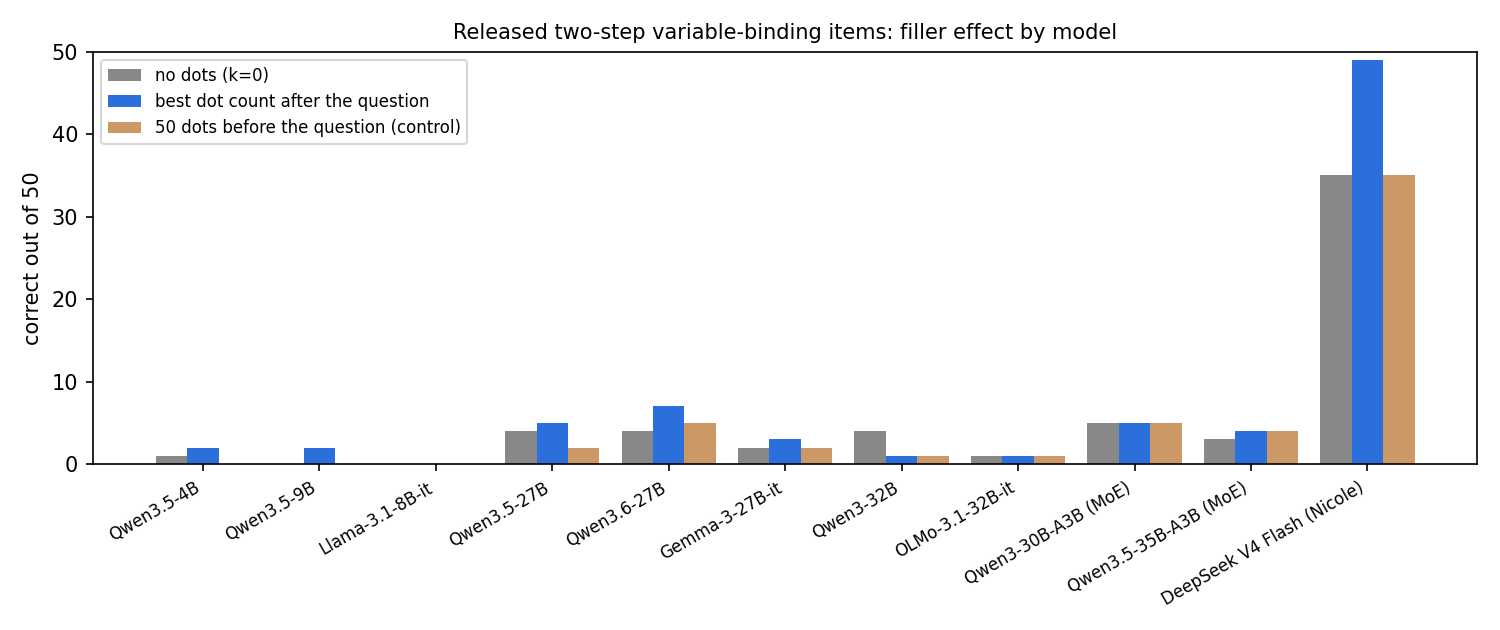
\includegraphics[width=\textwidth]{screen.png}
\caption{Correct out of 50 released two-step items for each model without dots, at the best dot count after the question, and with fifty dots before the question. DeepSeek V4 Flash (Nicole's result) is on the right for comparison.}\end{figure}

\begin{table}[h]\centering\small
\begin{tabular}{llrrrr}\toprule
Model & Type & $k=0$ & best dots & control & smallest $p$ \\ \midrule
DeepSeek V4 Flash (Nicole) & MoE, 4-stream residual & 35 & 49 & 35 & $1.2\times10^{-4}$ \\ \midrule
Qwen3.5-4B & dense & 1 & 2 & 0 & 1 \\
Qwen3.5-9B & dense & 0 & 2 & 0 & 0.5 \\
Llama-3.1-8B-Instruct & dense & 0 & 0 & 0 & 1 \\
Qwen3.5-27B & dense & 4 & 5 & 2 & 1 \\
Qwen3.6-27B & dense & 4 & 7 & 5 & 0.375 \\
Qwen3-32B & dense & 4 & 1 & 1 & 0.125 (dots hurt) \\
Gemma-3-27B-IT & dense & 2 & 3 & 2 & 1 \\
OLMo-3.1-32B-Instruct & dense & 1 & 1 & 1 & 1 \\
Qwen3-30B-A3B & MoE, 3B active & 5 & 5 & 5 & 1 \\
Qwen3.5-35B-A3B & MoE, 3B active & 3 & 4 & 4 & 1 \\ \bottomrule
\end{tabular}
\caption{Released two-step items, correct out of 50. ``Control'' is fifty dots placed before the definitions and question. The last column is the smallest exact McNemar $p$ across the five dot counts.}\end{table}

Every model is at floor. The best movement anywhere is Qwen3.6-27B going from 4 to 7 at two dot counts (4 helped, 1 hurt, $p = 0.375$, one of five lengths tested). Qwen3-32B and Qwen3-30B-A3B get worse with dots, in both placements.

The failures are not noise. Outputs are clean numbers. The smaller models emit a wrong number of roughly the right size; the 27B models get close (Qwen3.5-27B has a median error of 8 to 10 and more than half its answers within 10 of correct) without being right. Dots change the emitted answer in 80 to 90\% of items for every model. They perturb without steering.

Two facts show the failure is about direct-answer mode, not capability. With chain-of-thought enabled, Qwen3.5-9B solves 3/3, Llama 4/5, Qwen3.5-27B 5/5. And the plain arithmetic ``compute $2 \cdot 97 - 21$, then twice that plus 28'' gets \ttt{186} from the 9B and \ttt{370} from the 27B (correct: 374). The models cannot do two dependent steps in one forward pass at these sizes, so there is no partial circuit for filler to help.

\subsection{Log-probability and pass@$n$}

Accuracy on 50 items is coarse. The paired log-probability of the correct answer is not, and it agrees.

\begin{table}[h]\centering\footnotesize
\begin{tabular}{lrrr}\toprule
Model & best $\Delta \log p$ after question & $\Delta \log p$, control & $E[\text{pass@20}]$, $k=0 \to$ best \\ \midrule
Qwen3.5-27B & $+0.08$ (27/23 items up/down, $p=0.32$) & $-0.09$ & $0.47 \to 0.50$ \\
Qwen3.5-35B-A3B & $+0.00$ & $+0.33$ & $0.20 \to 0.21$ \\
Qwen3.6-27B & $+0.13$ ($p=0.67$) & $-0.05$ & $0.51 \to 0.52$ \\
Qwen3-32B & $+0.95$ ($p=0.67$) & $+0.05$ & $0.20 \to 0.26$ \\
Qwen3-30B-A3B & $-0.12$ & $-0.11$ & $0.23 \to 0.23$ \\
Gemma-3-27B-IT & $+1.22$ ($p=0.20$) & $+3.08$ (40/10) & $0.04 \to 0.06$ \\
OLMo-3.1-32B & $+1.25$ (36/14, $p=0.003$) & $+0.75$ & $0.10 \to 0.14$ \\ \bottomrule
\end{tabular}
\caption{Mean change in $\log p(\text{correct})$ versus $k=0$, best dot count, against the pre-question control at $k=50$.}\end{table}

Gemma's gain with dots is smaller than its gain with dots before the question, so it is a context-length effect. OLMo at $k=100$ is the only placement-specific cell in the whole screen, about half a nat net, on an answer whose median rank is in the fifties. Nothing here would survive sampling: pass@20 stays between 0.04 and 0.52 and moves by a point or two.

\subsection{An easier task does not help}

The released items are all one hidden hop before the final operation. I generated a one-step variant (\ttt{scripts/build\_onestep\_varbind\_configs.py}): same scaffold and vocabulary, five definitions with derived-expression distractors, but the queried variable is a literal, so the answer needs one hidden step. This puts the small models at 50 to 85\% and the 30B models at 82 to 100\%. Dots still do nothing. Qwen3.5-4B showed a 37 to 42 bump at five dots on 50 items (6 helped, 1 hurt, $p = 0.125$); on 200 fresh items it was 147 to 145, with helped and hurt within two of each other at every dot count, and the pre-question control slightly negative (4 helped, 12 hurt). That bump was noise.

\section{Part II: training a model to use the dots}

Since no open model does this out of the box, the next step was to make one. The design question is how to tell ``the model uses the dots'' apart from ``the model learned the task.'' The answer is to train with a mix of dot counts, including zero, and watch whether accuracy at $k=0$ stays behind accuracy with dots. DeepSeek looks like that: 70\% at $k=0$, 98\% at $k=50$.

\subsection{Data and recipe}

4,000 synthetic chain-length-1 items (\ttt{scripts/build\_varbind\_sft\_data.py}) matched to the released distribution: one to four literals, all coefficients ``twice,'' constants 1 to 30, derived expressions pointing at another derived variable 37\% of the time, and every released item excluded by signature. Each item is rendered once per epoch at a dot count drawn from $\{0, 5, 10, 25, 50, 100\}$. Only the answer tokens and the end-of-turn token carry loss; the prompt, demonstrations, and dots are context. LoRA rank 32 on all linear layers, learning rate $10^{-4}$ with cosine decay, effective batch 16, 500 optimizer steps (two epochs). Every 100 steps the adapter is evaluated on the released 50 items at every dot count and on the pre-question control, with the same code as the screen. Records are in \ttt{results/qwen3.5-9b/lora-*/} and \ttt{results/qwen3.5-4b/lora-mixedk/}.

\subsection{Five runs, one outcome}

\begin{figure}[h]\centering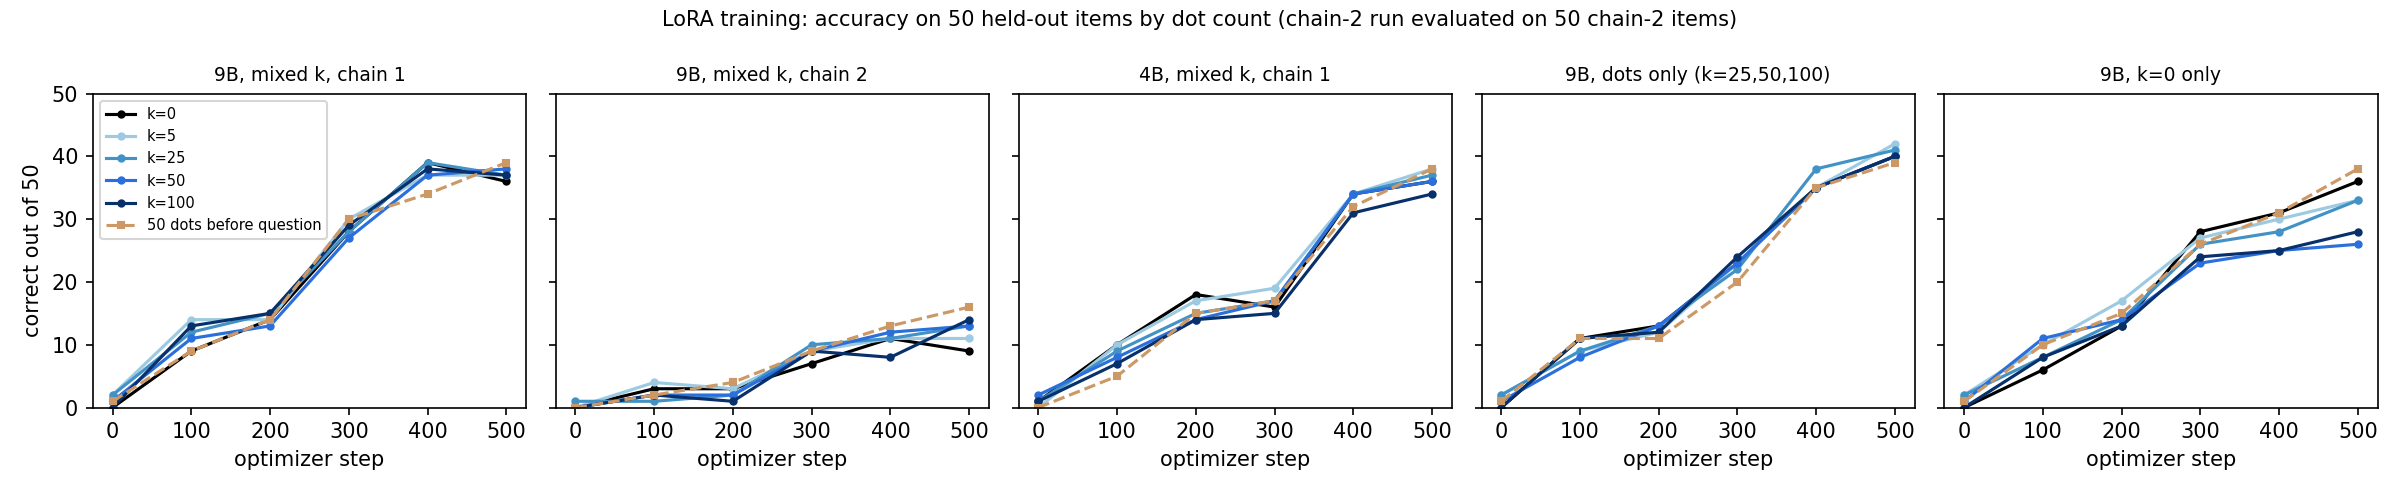
\includegraphics[width=\textwidth]{training.png}
\caption{Accuracy every 100 steps for the five training runs. Solid lines are dot counts after the question; the dashed line is fifty dots before the question. A model that used dots as a workspace would show the $k=0$ line staying below the others. None does.}\end{figure}

\begin{table}[h]\centering\small
\begin{tabular}{llrrrr}\toprule
Run & trained on & $k=0$ & $k=50$ & $k=100$ & control \\ \midrule
Qwen3.5-9B, chain 1 & $k \in \{0,5,10,25,50,100\}$ & 36 & 38 & 37 & 39 \\
Qwen3.5-9B, chain 2 & mixed $k$ (harder task) & 9 & 13 & 14 & 16 \\
Qwen3.5-4B, chain 1 & mixed $k$ & 36 & 36 & 34 & 38 \\
Qwen3.5-9B, chain 1 & dots only, $k \in \{25,50,100\}$ & \textbf{40} & 40 & 40 & 39 \\
Qwen3.5-9B, chain 1 & $k = 0$ only & 36 & \textbf{26} & 28 & 38 \\ \bottomrule
\end{tabular}
\caption{Correct out of 50 at step 500. The chain-2 run is evaluated on 50 held-out chain-2 items.}\end{table}

The mixed-$k$ run learns the task (0 to 72\%) and learns it uniformly. The only moment dots led was step 100 (9 at $k=0$ versus 11 to 14 with dots, control 9), and it closed by step 200. A 9B model fits the two-step chain in one forward pass, so mixed supervision gives it no reason to route through the dots.

I tried making the direct computation not fit by adding a hop (chain length 2, three sequential affine steps). The model learns slowly (18 to 28\% at step 500) and the only dot effect is again larger with dots \emph{before} the question (16) than after (13 to 14). I tried a smaller model (Qwen3.5-4B) on the theory that it might not fit two steps. It matches the 9B exactly.

The paired design settles it. The model trained only on prompts with dots, which never saw a dotless prompt, scores 40/50 without dots. Whatever it learned lives outside the dot positions. The mirror image, the model trained only without dots, loses ten items when dots are inserted after the question (14 hurt, 4 helped at $k=50$) and none when they are inserted before it. For an untrained-on-dots model the dots are interference at the answer position. Training with them present teaches the model to make them inert, not to use them.

\section{Part III: is the trained model using the dots at all?}

Everything in this section is on held-out items the trained model never saw and that were not used to pick a checkpoint. The model under study is the dots-only adapter, which is the strongest ``good with dots'' model (80\% on the released items, 67 to 73\% on 100 held-out items at every dot count).

\begin{figure}[h]\centering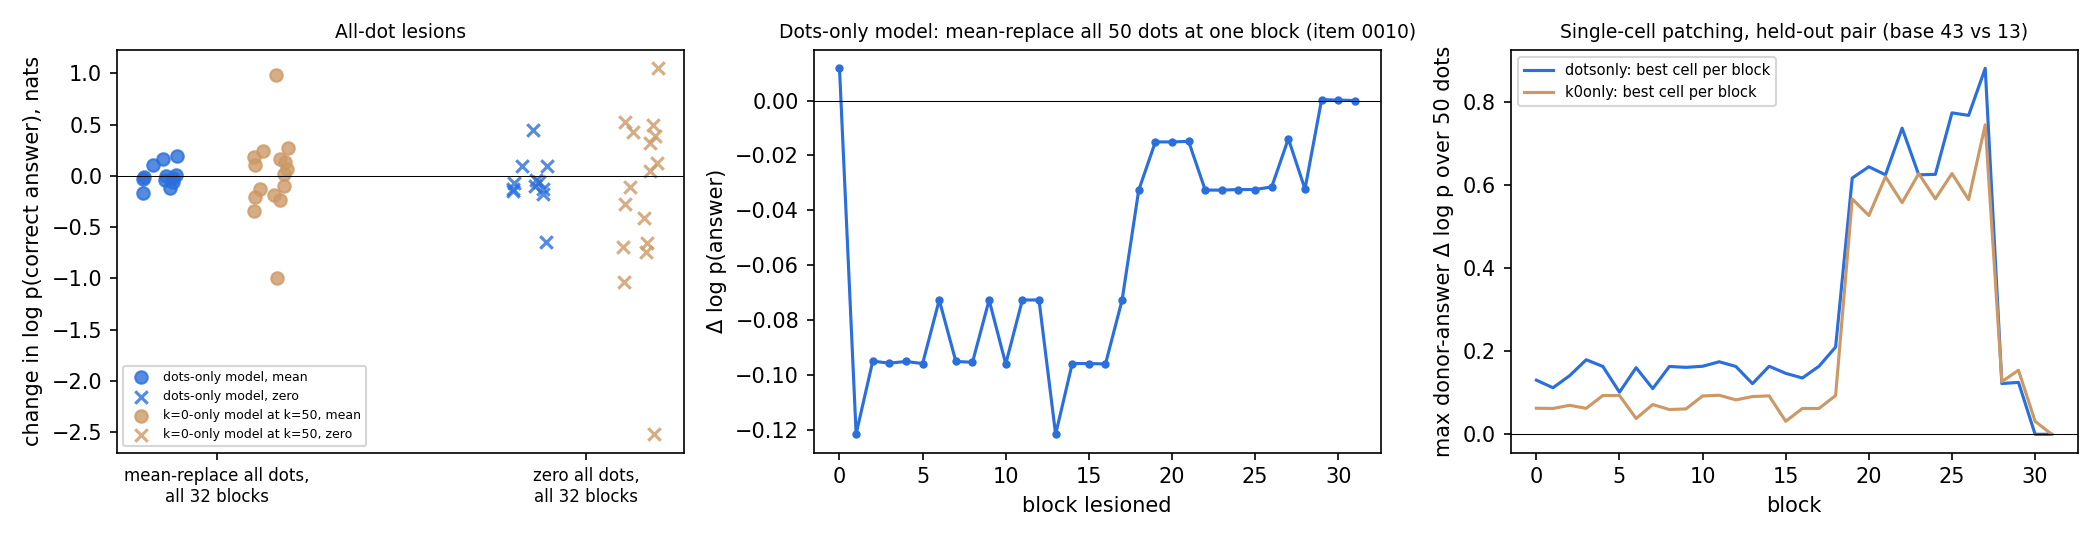
\includegraphics[width=\textwidth]{causal.png}
\caption{Left: change in $\log p(\text{answer})$ when every dot residual is replaced at all 32 blocks at once, per item. Middle: same replacement at one block at a time, one item. Right: single-cell patching of donor dot residuals into a target prompt, best cell per block, for a held-out pair differing in one prompt token.}\end{figure}

\subsection{Lesions: wipe every dot at every block}

\ttt{scripts/patch\_varbind\_hf.py -{}-lesion-all-dots -{}-lesion-all-layers} replaces all 50 dot residuals with their mean over positions (or with zeros) at all 32 decoder blocks simultaneously, so no later block can re-read pre-lesion dot content. On twelve items the dots-only model gets right at $k=50$, the mean lesion shifts $\log p(\text{answer})$ by a median of $-0.02$ nats (range $-0.17$ to $+0.20$) and changes one greedy output, to the correct answer. Zeroing everything shifts the median by $-0.09$ and leaves 11 of 12 correct.

The lesion has teeth. On the $k=0$-only model at $k=50$, where dots hurt behaviorally, the same intervention swings $\log p$ by up to $\pm 1$ nat (mean) or $\pm 2.5$ (zero), changes four to eight of sixteen greedy outputs, and repairs two to three wrong answers. Dot content is causally live in that model, as interference.

\subsection{Patching: 1,600 single cells}

From held-out item 0067 ($43 \to 99 \to 198 \to 203$) I built a one-digit counterfactual ($13 \to 39 \to 78 \to 83$) whose prompt differs at exactly one token. The dots-only model answers all 18 members of the family correctly except two near misses. Patching the donor's dot residual into the target one cell at a time over 32 blocks $\times$ 50 dots, the donor answer 83 starts at $\log p = -20.5$ and the best single cell adds 0.88 nats. The target answer never drops more than 0.03. Nicole's DeepSeek pair gave 4.9 nats from one cell. The only structure is a band at blocks 19 to 27 where the best cells reach 0.6 to 0.9 nats, matching the faint late leak in the lens grids below.

\subsection{Logit-lens grids}

Eight held-out items at $k=50$ (the five the dots-only model gets right only with dots, plus three it gets right either way and whose stage values have distinct first digits), each with Nicole's stage-matched derangement controls, for the dots-only, $k=0$-only, and base models. Grids cover all 32 blocks at all 50 dots plus the answer cue and generation position; final-block closure error is 0.0 everywhere.

The dot positions carry nothing stage-specific by this readout. Rank-1 hits for true stage digits in filler cells (at most 3 of 8 items, at most 0.9 of 1,600 cells) match the control labels. Averaged over late-third filler cells, the true answer digit beats its control by 0.12 nats in the dots-only model and 0.36 in the $k=0$-only model, and by about zero in early and middle blocks. The top-1 token at a filler cell is a digit in 0.2\% of late cells; it is most often the dot token itself. At the generation position the answer's first digit is rank 1 at block 30 of 32 in 8/8 items. Viewers: \ttt{results/\allowbreak qwen3.5-9b/\allowbreak lens-heldout-k50/\allowbreak <model>/\allowbreak <item>/\allowbreak viewer.html}.

\section{Part IV: what a dot position is doing}

The lens can only see content along token directions. To see the rest I dumped every block's residual at all 50 dots, the last question token, the answer cue, and the generation position for 100 held-out items at $k=50$, for the base, dots-only, and $k=0$-only models, plus attention mass by prompt region in the eight full-attention blocks (\ttt{scripts/dump\_dot\_residuals\_hf.py}, \ttt{scripts/analyze\_dot\_residuals.py}). Qwen3.5 alternates Gated DeltaNet blocks, which are linear attention with no attention matrix, with full attention; the attention results cover the eight full-attention blocks only.

\subsection{A dot residual is almost entirely ``I am dot number $k$''}

\begin{table}[h]\centering\small
\begin{tabular}{lccc}\toprule
Model & var.\ by position & var.\ by problem & cos, same dot, other problems \\ \midrule
base & 0.69 / 0.51 / 0.48 & 0.01 / 0.01 / 0.02 & 0.92 / 0.83 / 0.81 \\
dots-only & 0.88 / 0.74 / 0.60 & 0.01 / 0.02 / 0.05 & 0.99 / 0.99 / 0.97 \\
$k=0$-only & 0.82 / 0.63 / 0.46 & 0.01 / 0.06 / 0.10 & 0.98 / 0.88 / 0.88 \\ \bottomrule
\end{tabular}
\caption{At blocks 16 / 24 / 31: fraction of dot-residual variance explained by dot position versus by problem, and cosine similarity of the same dot position across different problems.}\end{table}

Which problem precedes the dots explains 1 to 5\% of the dot residuals' variance in the dots-only model. The same dot position in two different problems has cosine 0.97 at the last block. Training with dots made the dots \emph{more} problem-independent than in the base model (0.81 there); training without them left them less so (0.88) and gave problem identity its largest share (10\%).

\subsection{The small problem-dependent part is a selective copy of the relevant numbers}

\begin{figure}[h]\centering
\includegraphics[width=\textwidth]{probes.png}
\caption{Ridge probes (5-fold cross-validation over items) predicting stage values from the mean dot residual, the last question token, the answer cue, and the generation position, by block. Dashed lines are shuffled-label controls.}\end{figure}

Ridge probes read the queried chain's base literal from the mean dot residual at $R^2 = 0.98$ in the dots-only model (0.43 in the base), the chain's constants at 0.92 to 0.96, and the answer at 0.97. A visible literal that is \emph{not} on the queried chain is not decodable ($R^2 \le 0.06$ after block 20). So the dots do reflect variable-binding resolution: they encode which numbers matter. Two qualifications. On an affine task the answer is a linear function of the inputs, so a linear probe cannot distinguish stored inputs from a computed answer, and ``answer $R^2 = 0.97$'' is not evidence the dots computed anything. And the same information sits at the answer cue at $R^2 = 0.99$ in every model. This is a faint redundant copy that nothing downstream reads, and fine-tuning sharpened it everywhere whether or not dots were in the training prompts (the $k=0$-only model's dots reach the same $R^2$).

\subsection{The answer positions do not look at the dots}

\begin{figure}[h]\centering
\includegraphics[width=\textwidth]{attention_heatmaps.png}
\caption{Attention mass by key region in the eight full-attention blocks, mean over heads and 100 items. Regions: BOS, prefix (system sentence and demonstrations), the target problem, the dots, and the answer template.}\end{figure}

The dots-only model's answer cue and generation position put 1 to 4\% of their attention on the 50 dots in every full-attention block. The base model's answer cue puts 18\% there at block 23, and the $k=0$-only model, which is hurt by dots, 12 to 13\%. The single head most attentive to dots at the generation position reaches 0.08 in the dots-only model, 0.18 in the base, 0.24 in the $k=0$-only model. Training with dots taught the answer positions to look away from them.

The dots themselves attend mostly to the few-shot demonstrations (50 to 84\% of mass), then to each other (20 to 28\% at the last block), and to the target problem only in the middle blocks (a 37\% peak at block 11 in the dots-only model).

\subsection{The dots are processed, toward predicting the next dot}

\begin{figure}[h]\centering
\includegraphics[width=\textwidth]{independence_trajectories.png}
\caption{By block: fraction of dot-residual variance explained by problem versus by position; logit-lens entropy at dots and at the generation position; residual norm at dots and at the generation position.}\end{figure}

Logit-lens entropy at dot positions falls from 11.2 nats at block 0 to 0.02 nats at block 31 in the dots-only model, versus 0.14 at the generation position. Residual norms grow along the same curve as content tokens. Each dot spends its depth becoming certain that the next token is a dot. That is work, but it is not the task's work.

\subsection{Summary of the anatomy}

A dot position in the fine-tuned model holds a dominant position-identity vector, a faint linear copy of the queried chain's numbers that is present more strongly at the answer cue, attends to the demonstrations and to other dots rather than to the problem, receives 1 to 4\% of the answer positions' attention, and predicts ``dot.'' Fine-tuning with dots present made the dots more uniform and less attended than in the untrained model. This is the opposite of a workspace. It also explains why dots hurt the model trained without them: its answer cue attends to dot content three to four times more, and that content is out of distribution.

\section{Part V: the same anatomy on DeepSeek V4 Flash}

With a 4$\times$H100 box I reran the dot-position analysis on the model that shows the behavioral effect, using Nicole's converted checkpoint and loader (her sanity gate passed: final-head closure and the lens identity anchor are exact). Fifty held-out items at $k=50$; every block's raw four-stream residual at all 50 dots, the last question token, the answer cue, and the generation position; and attention recomputed from $q$, $k$, the indexer's selection, and the per-head sink at every block, because the fused sparse-attention kernel returns no weights (\ttt{scripts/dump\_dot\_residuals\_dsv4.py}, \ttt{scripts/dump\_dot\_attention\_dsv4.py}).

Two architecture facts frame the attention numbers. Every V4 block sees a 128-token sliding window of raw keys plus compressed keys: 4-token blocks chosen by a learned indexer in even blocks 2 to 40, 128-token blocks in odd blocks 3 to 41; blocks 0, 1, and 42 are window-only. At our prompt lengths the indexer's top-512 is every block, so sparsity never bites. For the answer positions the dots are about 40\% of the raw window keys, and the demonstrations and most of the problem are reachable only through compressed keys.

\subsection{DeepSeek's answer positions look at the dots}

\begin{figure}[h]\centering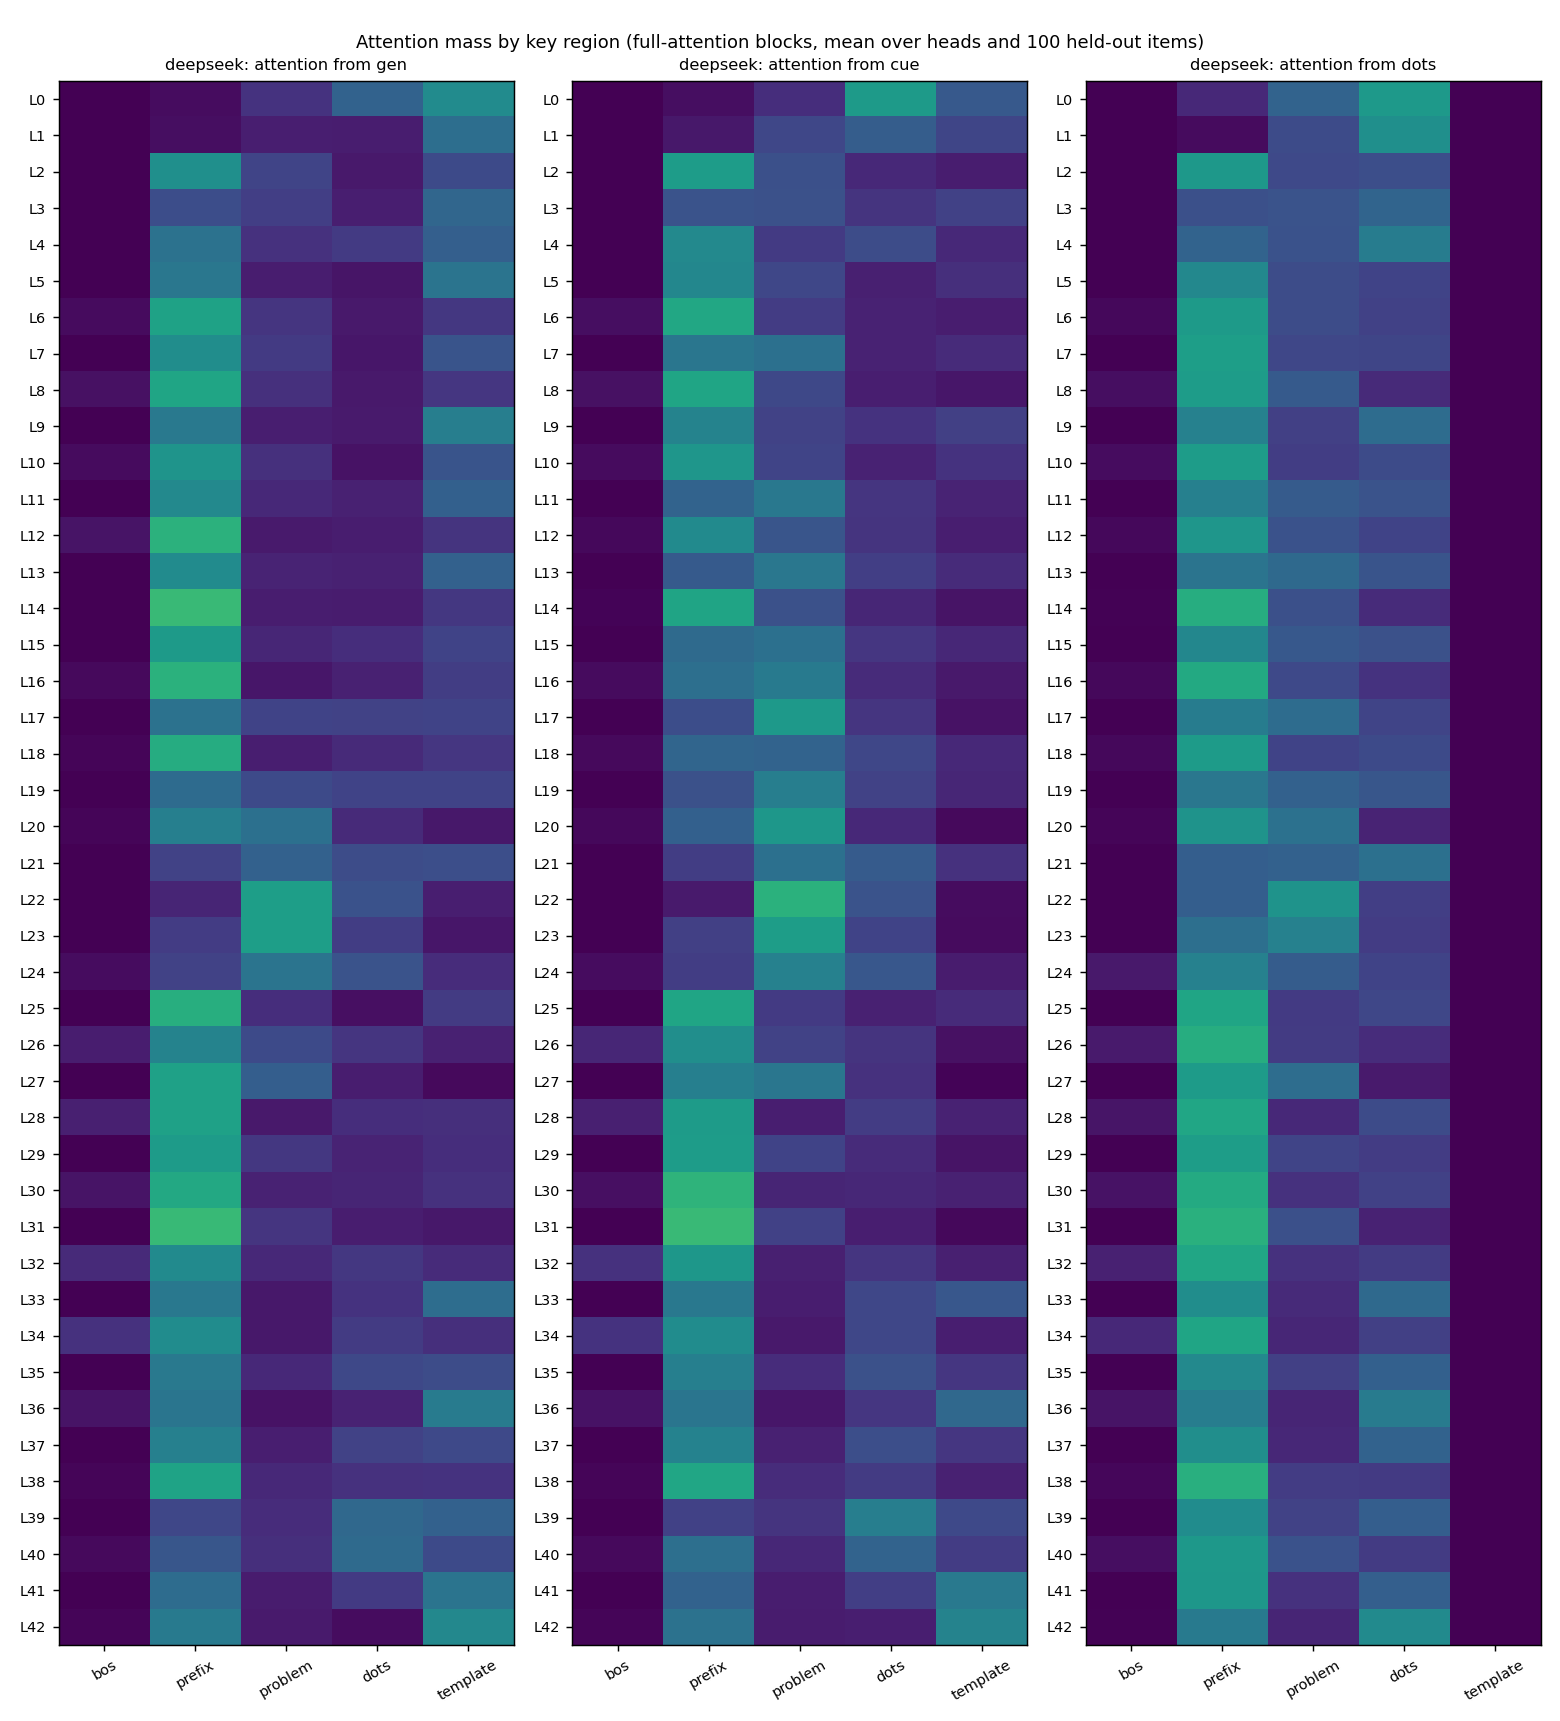
\includegraphics[width=0.85\textwidth]{deepseek_attention_heatmaps.png}
\caption{DeepSeek V4 Flash: attention mass by key region at every block, mean over 64 heads and 50 held-out items, from the generation position, the answer cue, and the dots.}\end{figure}

\begin{table}[h]\centering\small
\begin{tabular}{lrrrr}\toprule
Model & gen $\to$ dots & cue $\to$ dots & dots $\to$ dots & max head, gen $\to$ dots \\ \midrule
Qwen3.5-9B base & 0.010 & 0.046 & 0.13 & 0.18 \\
Qwen3.5-9B dots-only & 0.009 & 0.029 & 0.14 & 0.09 \\
Qwen3.5-9B $k=0$-only & 0.043 & 0.067 & 0.18 & 0.24 \\
\textbf{DeepSeek V4 Flash} & \textbf{0.164} & \textbf{0.195} & \textbf{0.26} & \textbf{0.90} \\ \bottomrule
\end{tabular}
\caption{Mean attention mass on the dot region over the last third of attention blocks, and the single most dot-attentive head at the generation position.}\end{table}

DeepSeek puts 20\% or more of the generation position's attention on the dots in blocks 21, 22, 24, 35, 39, and 40 (peak 0.35 at block 40), and of the answer cue's attention in fourteen blocks (peak 0.43 at block 39). Single heads reach 0.5 to 0.9 of their mass on dots in blocks 26 to 40. The dots attend to each other at 0.30 to 0.48 in blocks 33 to 42. The sliding window makes the dots cheap to reach, but Qwen had every token in reach and spent 1 to 4\% on them; DeepSeek spends 16 to 43\% in the blocks where Nicole's lens saw the ladder resolve.

\subsection{The dots are problem-specific, and the four streams divide the work}

Cosine of the same dot position across different problems at three-quarters depth is 0.78 in DeepSeek against 0.99 in the trained Qwen (0.83 in the Qwen base, 0.88 in the $k=0$-only model); the problem explains 4 to 5\% of late-block dot variance (Qwen dots-only: 2\%). Per hyper-connection stream:

\begin{table}[h]\centering\small
\begin{tabular}{lccc}\toprule
Stream & var.\ by problem (blocks 32 / 40) & cos, same dot, other problems & norm at dots, block 40 \\ \midrule
0 & 0.06 / 0.09 & 0.51 / 0.61 & 186 \\
1 & 0.03 / 0.03 & 0.68 / 0.79 & 286 \\
2 & 0.09 / 0.10 & 0.48 / 0.64 & 273 \\
3 & 0.02 / 0.05 & 0.88 / 0.76 & 49 \\ \bottomrule
\end{tabular}
\caption{DeepSeek V4 Flash dot residuals by hyper-connection stream.}\end{table}

Streams 0 and 2 carry the problem-specific content (cosine near 0.5, a tenth of their variance from problem identity). Stream 3 is the position-identity lane (cosine 0.88, small norm until the last blocks). Stream 1 is a high-norm carrier with little problem dependence. This is the first direct look at what the four lanes do at a filler position, and it fits the earlier guess that width lets a value be stored without overwriting the position's own state.

\subsection{Where the answer is computed}

\begin{table}[h]\centering\small
\begin{tabular}{lccc}\toprule
Model & answer $R^2$ from dots (mean) & from last question token & from answer cue \\ \midrule
Qwen3.5-9B dots-only & 0.97 & 0.94 & 0.99 \\
DeepSeek V4 Flash & 0.87 & \textbf{0.40} & 0.87 \\ \bottomrule
\end{tabular}
\caption{Best ridge-probe $R^2$ for the answer, by position.}\end{table}

In the trained Qwen the answer is already linearly present at the last question token, before any dot exists; the dots and the cue only repeat it. In DeepSeek the question token barely encodes it and the dots encode it as well as the answer cue does, consistent with the computation happening across the dot span rather than at the question. The affine-probe caveat applies to the absolute values, not to this contrast.

\begin{figure}[h]\centering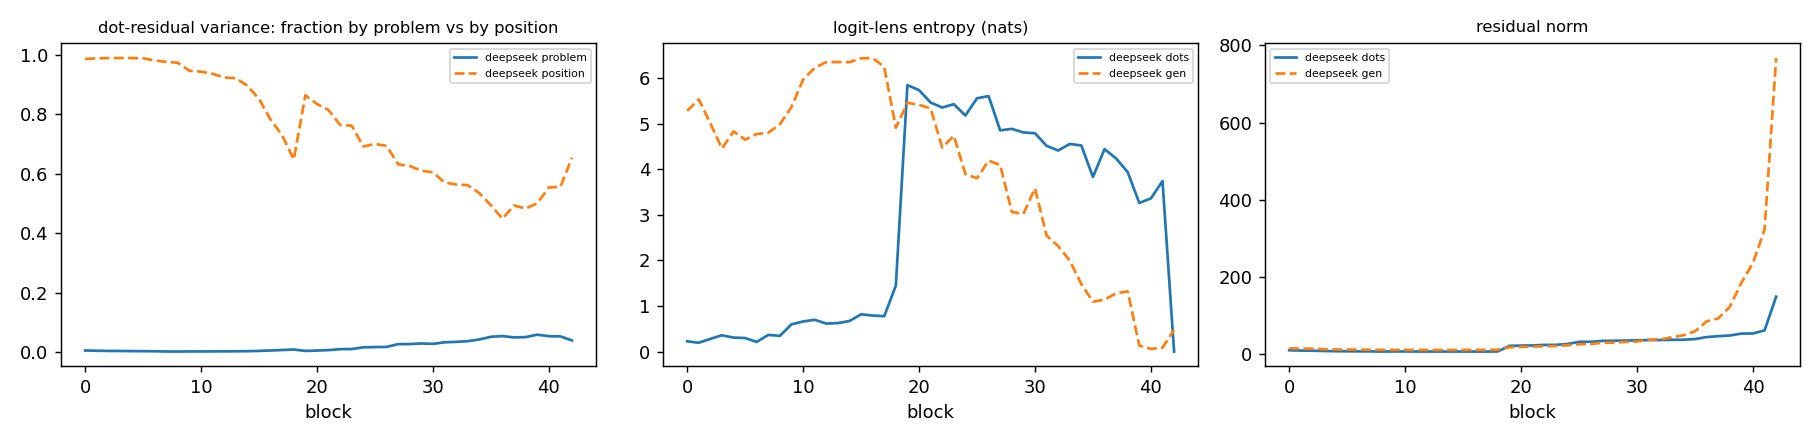
\includegraphics[width=\textwidth]{deepseek_independence_trajectories.png}
\caption{DeepSeek V4 Flash by block: fraction of dot-residual variance by problem versus position; logit-lens entropy (through Nicole's stream collapse) at dots and at the generation position; residual norm.}\end{figure}

One more difference. Logit-lens entropy at dot positions is 0.2 to 1.5 nats in blocks 0 to 18, jumps to 5.9 at block 19, and declines to 0 by block 42; Qwen's dots sit at 11 nats and only fall at the end. Whatever the early-block readout means under the stream collapse, the discontinuity at block 19 coincides with the first blocks where attention to dots exceeds 20\%.

\subsection{Summary}

On the model that shows the behavioral effect, the dot positions are attended (16 to 43\% late-block mass from the answer positions, single heads up to 0.9), problem-specific (cosine 0.78 across problems versus 0.99 in the trained Qwen), organized by stream (two content lanes, one position lane, one carrier), and hold the answer as strongly as the cue does while the question token does not. Every one of those is the opposite of what the fine-tuned Qwen showed. The base-checkpoint run that would say whether post-training installed this remains undone; the base weights (304\,GB FP8) exceed this box.

\section{Why does DeepSeek differ?}

I do not know, and the evidence mostly rules explanations out rather than in.

\paragraph{Scale.} Weakened. DeepSeek V4 Flash runs about 13B active parameters (256 experts, 6 active plus one shared, 43 blocks, width 4096), the same regime as the models tested. Total parameters (roughly 280B) is the only scale axis left, and it is confounded with everything else. The trained 9B is the sharper counterexample: it reached DeepSeek-level accuracy at $k=0$ (72\% versus 70\%) and got nothing from dots. Nicole's interpretation was that filler amplifies a circuit the model nearly has. The 9B nearly had the circuit and no amplification happened.

\paragraph{Architecture.} Partly ruled out. Two 3B-active mixture-of-experts models behave like the dense ones, so expert routing alone is not it. Three features unique to V4 among everything tested remain: the four-stream hyper-connection residual (four lanes per position to hold a value in without overwriting), multi-head latent attention, and a learned top-512 sparse attention index. The residual width is my candidate for why the habit \emph{works well} once a model has it: writing a value into another position without clobbering what is there is cheap with four lanes and expensive with one, and the $k=0$-only model shows the single-stream failure mode directly.

\paragraph{Post-training.} The leading suspect. Using dots means writing intermediate state into positions after the question and reading it back at the answer. No gradient in my training ever rewarded that, because the direct route always worked, and the learner takes the path that already exists. This matches Pfau et al.\ (2024), who found filler helps only when training makes it useful. DeepSeek V4 was trained hard with reinforcement learning to reason across a span of tokens before answering; a model that has internalized ``the span between question and answer is where thinking happens'' would plausibly treat any trailing tokens as thinking room. Nicole's readouts look like that: values staged by depth, broadcast across the span, read from the late band right before the answer. The awkward fact is that Qwen3.5 also has a thinking mode and shows nothing, so the difference would have to be in how each lab trained its non-thinking mode. Part V adds that whatever installed it, the result is visible in attention: DeepSeek's answer positions read the dots at 16 to 43\% while every Qwen variant, trained or not, reads them at 1 to 4\%.

\paragraph{The experiment that would decide.} \ttt{deepseek-ai/DeepSeek-V4-Flash-Base} is public and ungated: same architecture and pretraining, no post-training. If it shows the placement-specific gain, post-training is out. If it is flat, post-training built the behavior. It is 304\,GB of FP8 weights and needs an 8-GPU box, or a requantization to FP4 for Nicole's 4-GPU setup. The cheap partial check is DeepSeek-V2-Lite-Chat (2.4B active, no hyper-connections) on the existing harness.

\section{Limitations}

\begin{itemize}
\item Per-cell lens readouts on Qwen rank the first digit of a value, because the tokenizer splits digits. The derangement controls bound how much this could hide, and the probes and lesions do not depend on it, but a whole-number readout (Llama, DeepSeek) would be cleaner.
\item Linear probes cannot separate stored inputs from computed outputs on an affine task. The probe results say the dots encode the relevant numbers; they do not say the dots compute with them.
\item Twenty-four of thirty-two Qwen3.5 blocks are linear attention. Attention results cover the other eight. In the recurrent blocks the dots are recurrence steps regardless of content, so a structural ``extra compute'' from dots exists that the lesions remove the content of but not the steps.
\item The training phase shows that answer-only supervised fine-tuning with dots present does not induce workspace use in Qwen3.5 up to 9B. It does not show that no recipe can. Dense supervision on intermediate values placed in the dots, a task where a single forward pass provably cannot fit the computation, and reinforcement learning with a compute penalty are all untested.
\item The Llama weights are an ungated mirror (\ttt{unsloth/Llama-3.1-8B-Instruct}) of the gated Meta checkpoint. This does not affect behavioral numbers.
\item Fifty items is a small screen. The log-probability endpoint, the 100-item held-out sets, and the 200-item replication of the one bump that appeared are what make me confident in the nulls.
\end{itemize}

\section{What I would do next}

In order of information per GPU-hour:

\begin{enumerate}
\item Run DeepSeek-V4-Flash-Base on the released 50 items with the placement control. One afternoon on an 8-GPU box. Decides whether post-training or architecture is responsible.
\item Run DeepSeek-V2-Lite-Chat on the existing harness. Twenty minutes. Tests whether the DeepSeek training pipeline produces the effect without hyper-connections.
\item Train a model where dots are \emph{necessary}: a chain long enough that the direct computation cannot fit, with the loss also applied to intermediate values written at the dot positions during a first phase, then removed. If that produces a dot-dependent model, Nicole's causal ladder can be run on it and compared with DeepSeek's mechanism.
\item On the DeepSeek side, read the four residual streams separately. The unresolved question in Nicole's pipeline is how the released lens collapses four streams to one; values living in one lane may be invisible after the collapse, and her ``raw first product never appears'' result could be that artifact.
\end{enumerate}

\appendix
\section{Reproducibility}
\begin{raggedright}

All code is in the project repository. Model-touching scripts run on one GPU with \ttt{transformers} from main (Qwen3.5 requires it), \ttt{peft}, and PyTorch 2.11 with CUDA 12.8.

\begin{itemize}
\item Behavioral sweep: \ttt{scripts/\allowbreak extract\_hf.py -{}-phase eval} on any \ttt{configs/\allowbreak *\_dot\_length\_sweep.json}; \ttt{scripts/\allowbreak analyze\_behavior\_sweep.py} for tables; \ttt{scripts/\allowbreak screen\_models.sh} to loop models.
\item Data and training: \ttt{scripts/\allowbreak build\_varbind\_sft\_data.py} (\ttt{-{}-chain-len}), \ttt{scripts/\allowbreak build\_onestep\_varbind\_configs.py}, \ttt{scripts/\allowbreak train\_varbind\_lora.py} (\ttt{-{}-ks} selects the dot counts).
\item Readouts: \ttt{scripts/\allowbreak extract\_hf.py -{}-phase filler -{}-adapter}, \ttt{scripts/\allowbreak build\_artifacts.py} for viewers, \ttt{scripts/\allowbreak analyze\_hf\_lens\_grids.py} and \ttt{\_deep.py}, \ttt{scripts/\allowbreak select\_heldout\_lens\_cases.py}.
\item Causal: \ttt{scripts/\allowbreak build\_varbind\_counterfactuals\_hf.py}, \ttt{scripts/\allowbreak patch\_varbind\_hf.py} (single-cell grid; \ttt{-{}-lesion-all-dots [-{}-lesion-all-layers]}).
\item Anatomy: \ttt{scripts/\allowbreak dump\_dot\_residuals\_hf.py}, \ttt{scripts/\allowbreak dump\_dot\_residuals\_dsv4.py}, \ttt{scripts/\allowbreak dump\_dot\_attention\_dsv4.py}, \ttt{scripts/\allowbreak setup\_dsv4\_box.sh}, \ttt{scripts/\allowbreak run\_dsv4\_dot\_dump.sh}, \ttt{scripts/\allowbreak analyze\_dot\_residuals.py}, \ttt{scripts/\allowbreak probe\_extra\_targets.py}, \ttt{scripts/\allowbreak plot\_dot\_analysis.py}.
\item Results: \ttt{results/\allowbreak <model>/\allowbreak } per model; training under \ttt{results/\allowbreak qwen3.5-9b/\allowbreak lora-*}; lens grids under \ttt{results/\allowbreak qwen3.5-9b/\allowbreak lens-heldout-k50/\allowbreak }; lesions and patching under \ttt{results/\allowbreak qwen3.5-9b/\allowbreak lora-*/\allowbreak lesion-all-layers/\allowbreak } and \ttt{results/\allowbreak qwen3.5-9b/\allowbreak patch-heldout-0067/\allowbreak }; anatomy under \ttt{results/\allowbreak qwen3.5-9b/\allowbreak dot-dump/\allowbreak analysis/\allowbreak }. The 1.3\,GB residual dumps stay on the compute box.
\item Nicole's DeepSeek pipeline and results: \ttt{scripts/\allowbreak extract\_dsv4.py} and \ttt{reports/\allowbreak algorithm-exploration-findings.md}.
\end{itemize}
\end{raggedright}

\end{document}
